\begin{figure}[H]
\centering
\subfloat
{
	
\includegraphics[width=0.05\textwidth]{images/balls/0.png}
}
\hspace{0.4\textwidth}
\subfloat
{
	
\includegraphics[width=0.05\textwidth]{images/balls/8.png}
}

\subfloat
{
	
\includegraphics[width=0.4\textwidth]{images/ballhist/0}
}
\subfloat
{
	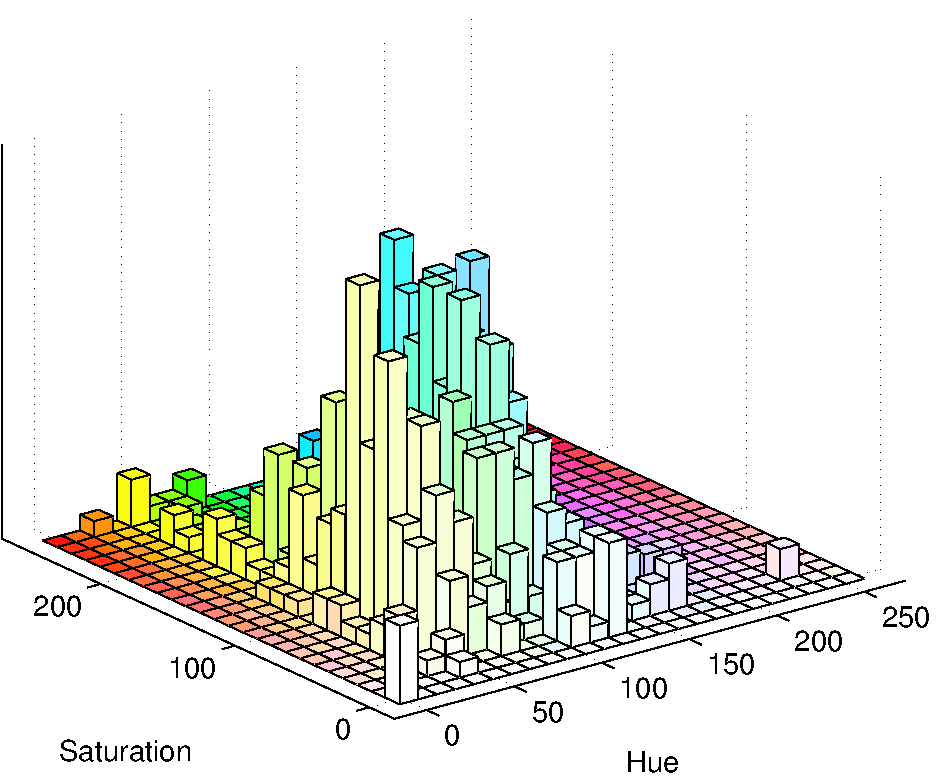
\includegraphics[width=0.4\textwidth]{images/ballhist/8}
}
\caption{Color histogram of cue and 8}
\label{fig:ballhist-cue-8}
\end{figure}
Figure \ref{fig:ballhist-cue-8} shows the histograms of the cue-ball and the 8-ball. The cue-ball distribution is isolated in a low-saturation area, having a yellow hue around 50. The saturation of the other balls is generally above the white saturation, making it possible to identify white pixels by setting a saturation threshold.

The hue-saturation distribution of the 8-ball is scattered all over the range. The reason for this, is that black is undefined in hue-saturation space. Black will have to be detected by the brightness value, which is significantly lower than other balls. \fxnote{VALUE HISTOGRAM HERE.}

\begin{figure}[H]
\centering
\subfloat
{
	
\includegraphics[width=0.05\textwidth]{images/balls/3.png}
}
\hspace{0.4\textwidth}
\subfloat
{
	
\includegraphics[width=0.05\textwidth]{images/balls/7.png}
}

\subfloat
{
	
\includegraphics[width=0.4\textwidth]{images/ballhist/3}
}
\subfloat
{
	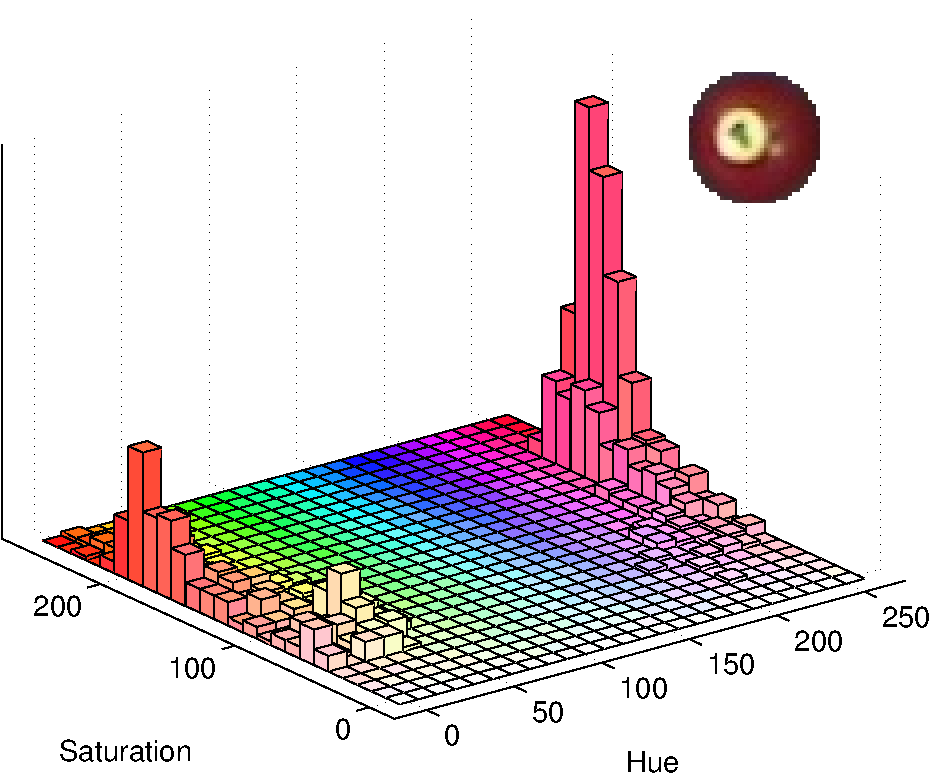
\includegraphics[width=0.4\textwidth]{images/ballhist/7}
}
\caption{Color histogram of 3 and 7}
\label{fig:ballhist-3-7}
\end{figure} 
Figure \ref{fig:ballhist-3-7} shows a situation where the balls are going to be difficult to separate. Depending on the lighting and camera settings, the color of 3, 5 and 7 have almost the same hue, and are only separable in saturation.

\begin{figure}[H]
\centering
\subfloat
{
	
\includegraphics[width=0.05\textwidth]{images/balls/1.png}
}
\hspace{0.4\textwidth}
\subfloat
{
	
\includegraphics[width=0.05\textwidth]{images/balls/5.png}
}

\subfloat
{
	
\includegraphics[width=0.4\textwidth]{images/ballhist/1}
}
\subfloat
{
	
\includegraphics[width=0.4\textwidth]{images/ballhist/5}
}
\caption{Color histogram of 1 and 5}
\label{fig:wrongcamera}
\end{figure} 


\begin{figure}[H]
\centering
\subfloat
{
	
\includegraphics[width=0.05\textwidth]{images/balls/2.png}
}
\hspace{0.4\textwidth}
\subfloat
{
	
\includegraphics[width=0.05\textwidth]{images/balls/4.png}
}

\subfloat
{
	
\includegraphics[width=0.4\textwidth]{images/ballhist/2}
}
\subfloat
{
	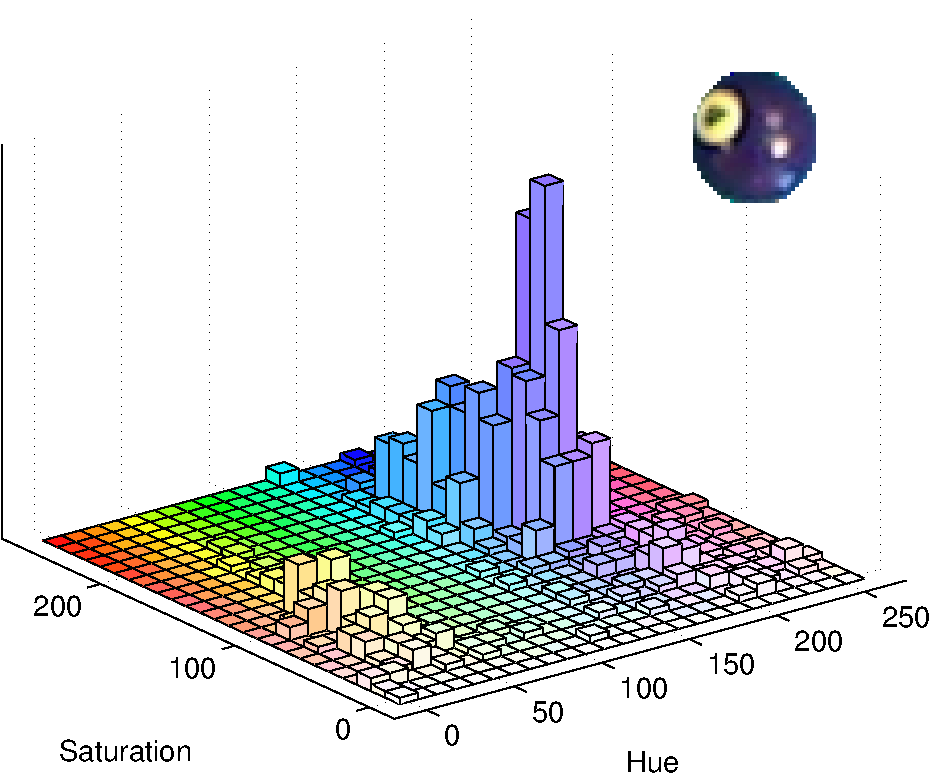
\includegraphics[width=0.4\textwidth]{images/ballhist/4}
}
\caption{Color histogram of 2 and 4}
\label{fig:wrongcamera}
\end{figure}